\chapter{Context} % (fold)
\label{cha:context}
In order to see what ubiquitous computing can do for people while they sleep, there must at least be a basic understanding of what sleep is. Sleeping consists of several states ~\cite{Silber:2007fk}, these states are described in the first section. The second section provides a description about what can be done using sleep state detection, this will be done using some existing examples of applications.
 
\section{Sleep States} % (fold)
\label{sec:sleep_states}
There are two broad sleep states: REM (Rapid eye movement) and NREM (non-rapid eye movement) sleep. Sleeping people go from REM to NREM sleep in cycles. The two main states are described first, followed by what the cycle looks like.

\subsection{REM Sleep} % (fold)
\label{sub:rem_sleep}
Rapid eye movement sleep is characterized by, unsurprisingly, by rapid movements of the eyes. There are two other important characteristics: the first characteristic is that other muscles are in a state of paralysis, meaning that people do not move anything besides their eyes during this state; the second characteristic is that there seems to be a lot of brain activity during this stage. On average, an adult will spend around $20$ to $25$ percent of their sleep in the REM state.

Dreaming usually occurs during this sleep state. This could explain why the eyes move rapidly, according to Leclair-Visonneau, et \emph{al}. ~\cite{LeclairVisonneau:2010:Brain:20478849} the eyes seem to move as if the dream is real. Dreaming can also explain why muscles are paralyzed during REM sleep, this would prevent people from accidentally hurting themselves by acting out their dreams.

The function of REM sleep is up to debate, there are multiple studies that suggest different function; for example, some studies suggest that REM sleep improves memory ~\cite{Marshall:2006:Nature:17086200} or creativeness ~\cite{Wagner:2004:Nature:14737168}. People wake up easily during REM sleep; i.e., it is a light sleep state. Detection of the REM state is interesting for two reasons: the first reason is that this seems like an opportune moment to wake someone up; the second reason, assuming that it is important to have enough REM sleep, is to keep track of the amount of REM sleep someone gets over multiple nights.
% subsection rem_sleep (end)

\subsection{NREM Sleep} % (fold)
\label{sub:non_rem_sleep}
Non-rapid eye movement sleep can be further divided into three states: \emph{N1}, \emph{N2} and \emph{N3}. The first two state can be characterized as light sleep and the third as deep sleep. This means that people are easily awakened during the first two stages. Not surprisingly, during these three stages there is little to no eye movement. It is very rare to dream during these stages, and the muscles are not paralyzed like during REM sleep. This means that it could be possible to make a distinction between REM and NREM by measuring movement; the least movement occurs during REM sleep.

The first state, \emph{N1}, is what people are in when they fall asleep. When woken up during this state, just after falling asleep, people may not even be aware that they have been asleep. This state, however, does not only occur just after falling asleep, an overview of the cycle of states is provided in the next section. Another interesting characteristic of the first state is that people experience hypnic jerks, brief and involuntary muscle twitching. Furthermore, it seem that a lack of sleep causes a more frequent occurrence of these hypnic jerks ~\cite{Sander:1998:J-Neurol-Neurosurg-Psychiatry:9598699}.

The second light sleep state, \emph{N2}, is the state that compromises most of the sleep ($45$ to $55$ percent). Muscle activity decreases during this state and people lose conscious awareness of their surroundings. This state usually occurs between the first and the third state and between the third state and REM sleep. People are easily awakened during this stage.

The worst time to wake up a person is during the third state, \emph{N3}, this state is also called deep sleep or slow-wave-sleep (SWS). When people are awakened during this stage, their mental performance is impaired for about half an hour. This impairment reduces peoples' cognitive awareness ~\cite{Tassi2000341}.
Deep sleep is the state in which people feel the need to go back to sleep, i.e., this is not the best time to wake someone up.
% subsection non_rem_sleep (end)

\subsection{Sleep Cycle} % (fold)
\label{sub:sleep_cycle}
There is a transition between states during sleep, this transition follows a certain cycle. Broadly speaking, there is a recurring transition between REM and NREM. Transitions between the NREM states also follows a recurring pattern. Image \ref{fig:images_sleep_cycle} show how this sleep cycle progresses.

\begin{figure}[htbp]
  \centering
    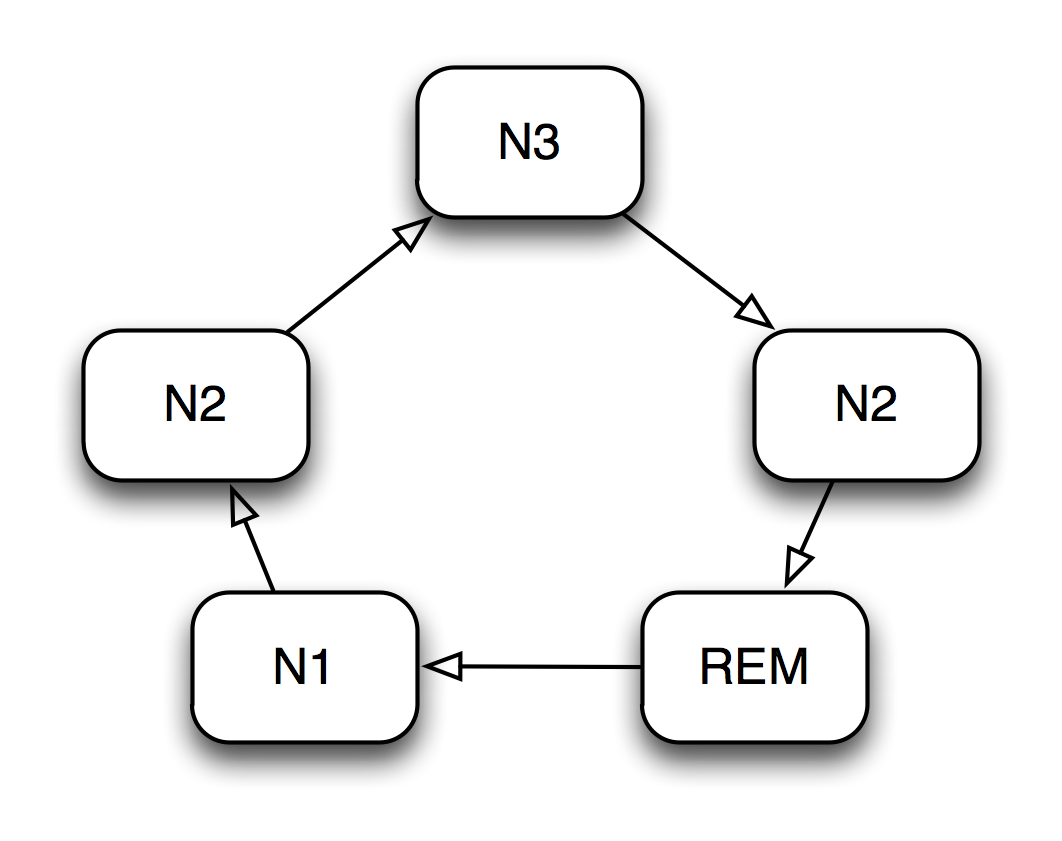
\includegraphics[scale=1]{images/sleep_cycle.png}
  \caption{Transition between sleep cycles}
  \label{fig:images_sleep_cycle}
\end{figure}

The sleep cycle starts in the N1 stage. The N2 stage occurs two times in the cycle; between N1 and N3, and between N3 and REM. After the REM state, a person returns to the N1 state. Not shown in Image \ref{fig:images_sleep_cycle} is that people may awaken for short periods during REM sleep.

An example of the transitions of states during sleep is provided in Image \ref{fig:hypnogram}. This image shows two important things: firstly, it shows that there are brief periods of awakening during sleep; secondly, it shows that the duration of the REM state becomes longer over time. This image also shows a fourth state; the third state used to be divided into two states, this is no longer the case ~\cite{Silber:2007fk}.

\begin{figure}[htbp]
  \centering
    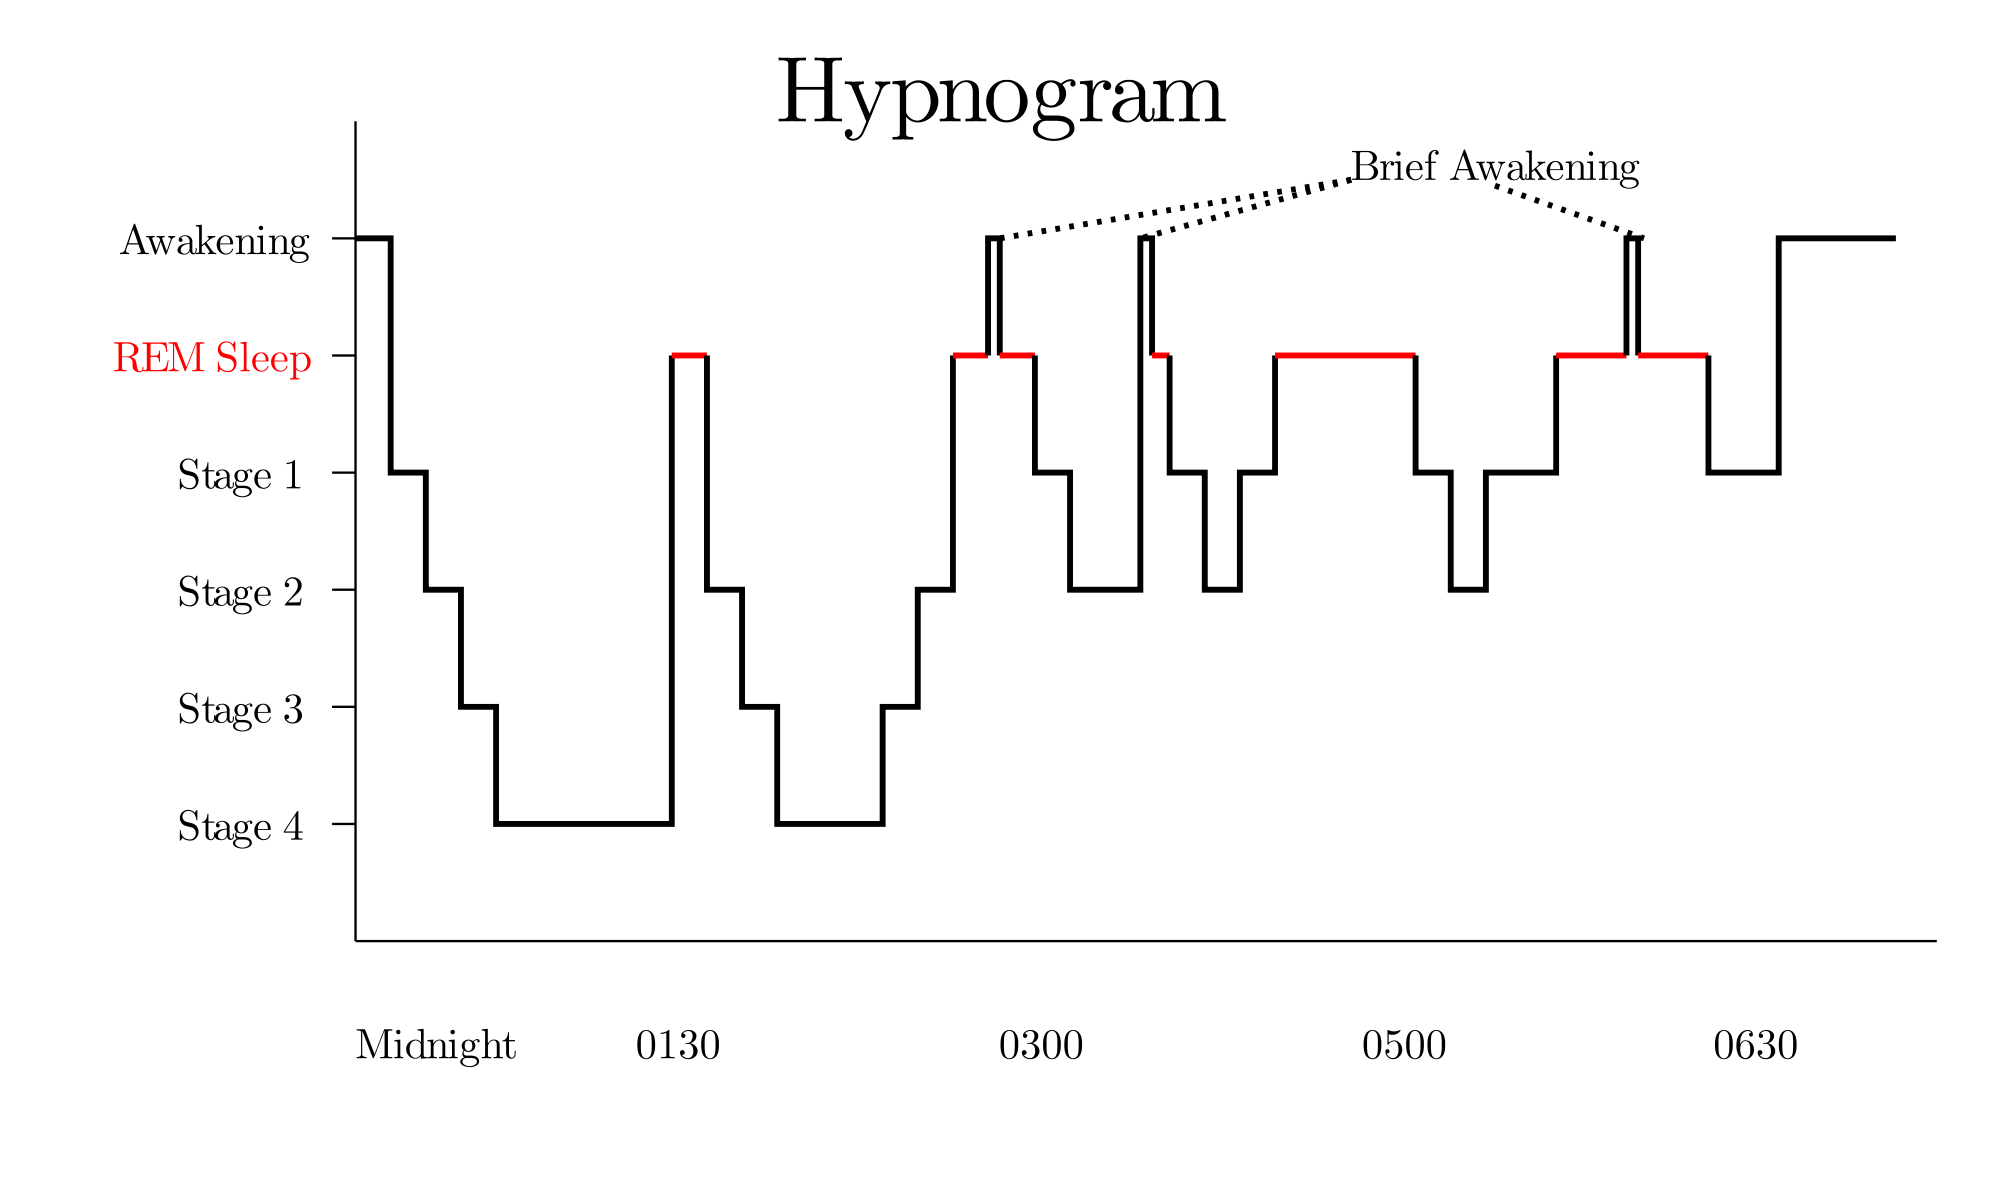
\includegraphics[width=\textwidth]{images/hypnogram.png}
  \caption{A hypnogram showing transition between sleep states ~\cite{RazerM:2011uq}}
  \label{fig:hypnogram}
\end{figure}
% subsection sleep_cycle (end)

% section sleep (end)

\section{Applications} % (fold)
\label{sec:applications}
Now that there is a better understanding about what sleep is and what its characteristics are, a closer look at what sleep state information can be used for is in order. The first application may be the most obvious, sleep state information can be used to wake people up at the moment they awaken most easily. The second application looks more at how sleep state information can be used in a larger ubiquitous computing system.

\subsection{Alarm Clock} % (fold)
\label{sub:alarm_clock}
Using information about sleep states to wake people up at the best moment is already being used. Applications that function as such a smart alarm clock already exist; for example, Sleep Cycle ~\cite{sleep-cycle} for the iPhone and Smart Alarm ~\cite{smart-alarm-clock} for Android phones.

These alarm clock applications use accelerometers in the phone to determine in what state people are in. These alarm clocks then try to wake up the user before a set time, when the most opportune sleep state occurs. After the set time, the alarm goes of anyway; this is to prevent someone from waking up too late.

There is no possibility to share information of the sleep state with other applications during sleep. Users are, however, able to view and share (via email of Facebook) graphs displaying the transitions between and duration of states (on the iPhone at least). Using this information in an overarching ubiquitous system would then not be very user friendly, since the user must share this information every day.
% subsection alarm_clock (end)

\subsection{Context Awareness} % (fold)
\label{sub:context_awareness}
Information about sleep states can also be useful in larger ubiquitous systems. Some research is already being done to this end, for example UbiSAS ~\cite{Yoon-Sik_Jae-Doo_2006}. An alarm clock, for example, could be a part of such a system. There are, however, more uses for sleep state information, some example will be described.

The amount of sleep people have, and the duration of the sleep states, can influence how people feel. If information about these states can be shared between components of an ubiquitous system, this system could, possibly, take someones state into account; for example, advising someone that he or she should go to sleep.

Information about going to sleep and waking up, not necessarily the sleep states, can also be of use. A ubiquitous system can, for example, adjust lighting according just prior to waking up or going to sleep. Ubiquitous systems can determine actions according to context, adding information about sleep and sleep states can, arguably, be valuable.
% subsection context_awareness (end)

% section applications (end)

% chapter context (end)